Detectie van kleuren kan binnen verschillende kleurruimten, in dit onderzoek zijn RGB en HSL gebruikt om de schakeringen te detecteren, in sectie \ref{sec:achtergrond} staat meer achtergrondinformatie hieromtrent. Een eerste bemerking in het verschil tussen RGB en HSL is dat HSL een betere detectieratio heeft voor alle kleuren, zie figuur \ref{fig:HSLvsRGB}. RGB herkent dan weer duidelijk beter het wit en het zwart. Dit verschil is toe te wijzen aan de restrictie op het herkennen van zwart en wit in HSL. De lichtsterkte moet ofwel kleiner dan 10 ofwel groter dan 90 zijn om respectievelijk zwart en wit te detecteren. Het is een strikte restrictie om beiden te herkennen.

Met uitzondering tot geel en cyaan zijn alle kleuren met een verschil van minstens 10\% beter herkent door HSL. Bij zowel groen, blauw, magenta als rood is HSL opmerkelijk beter. Deze kleuren gaan over, of leunen aan, 90\% detectieratio. De detectie van rood leunt zelfs aan tegen de 100\%.
Om kleuren te herkennen heeft HSL duidelijk een meerwaarde. Wit en zwart herkennen gebeurt best niet met een kleurdetectie, ze zijn vaak geïdentificeerd als een andere kleur, zie sectie \ref{subsec:kleuren} omtrent kleuren. Het contrast tussen deze twee is een betere keuze om ze te onderscheiden van elkaar.

\begin{figure}
	\center
	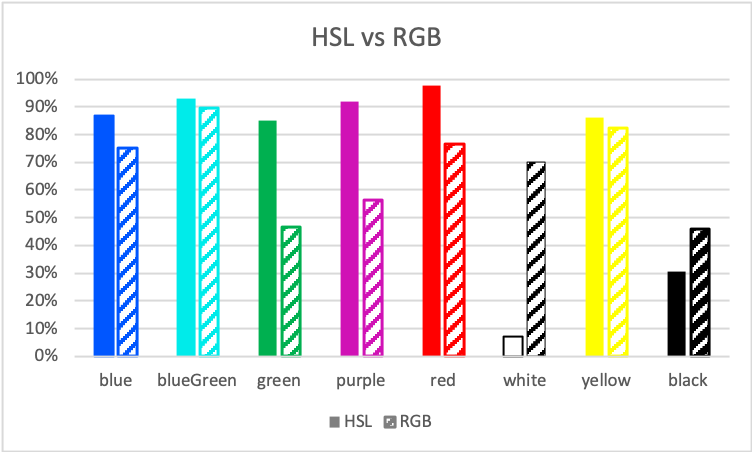
\includegraphics{img/HSLvsRGB}
	\caption{Verschil tussen juist gedetecteerde kleuren in HSL en RGB per kleur.}
	\label{fig:HSLvsRGB}
\end{figure}

				